\begin{figure}
    \begin{center}
    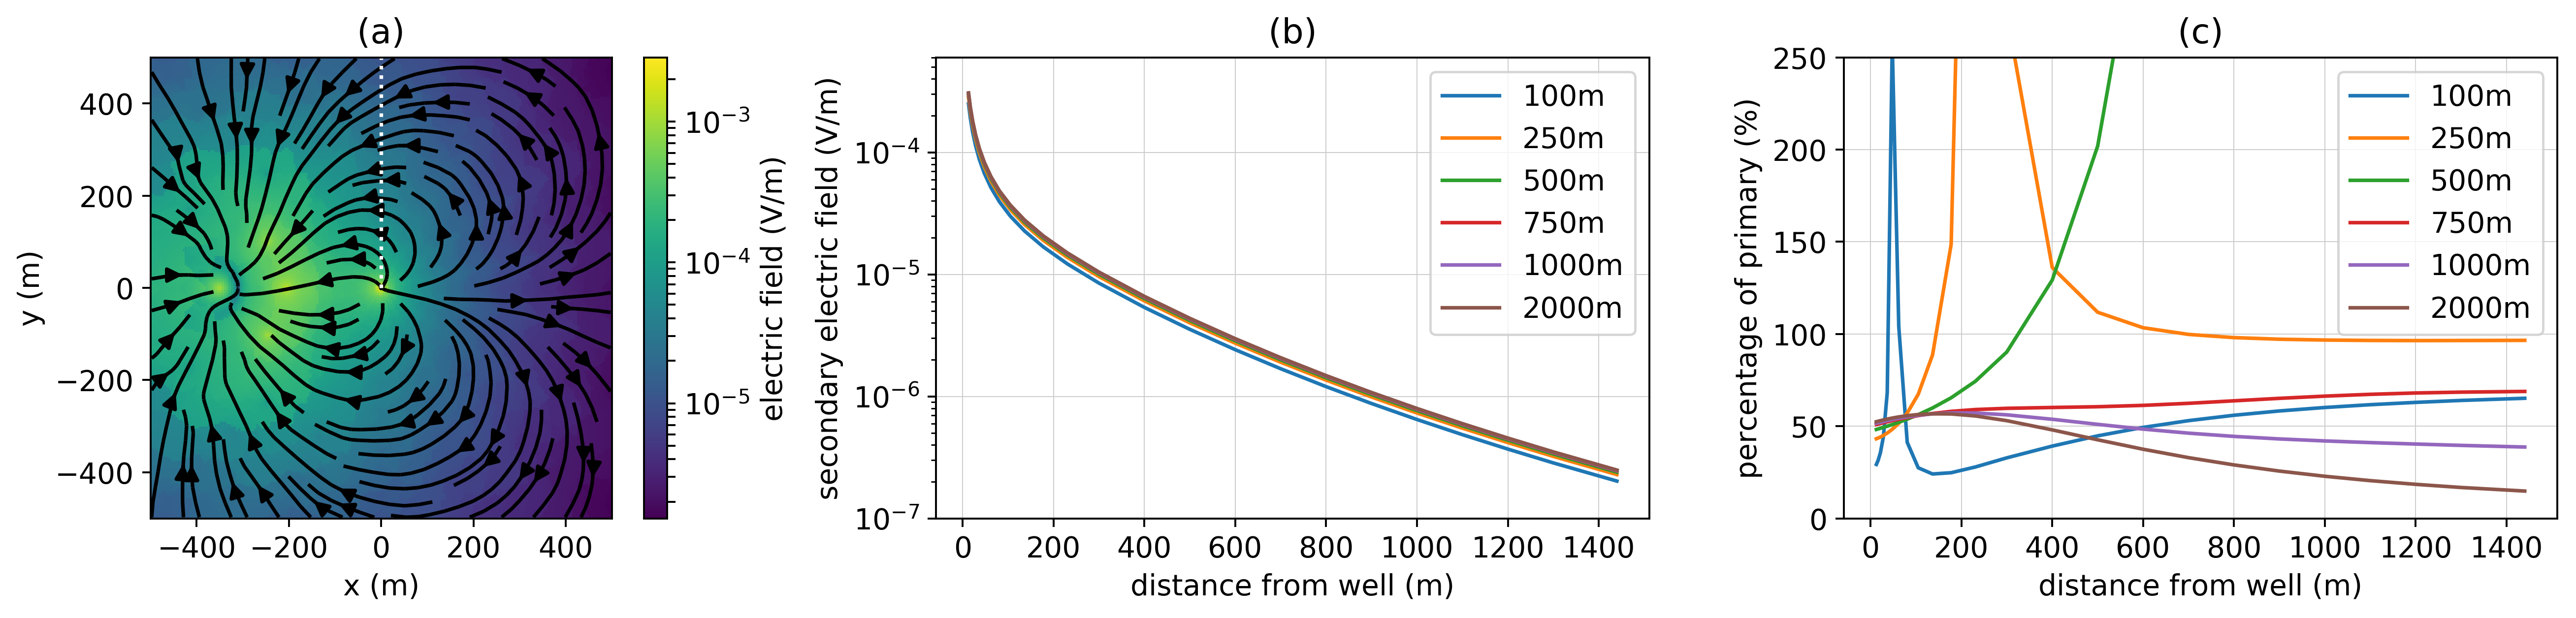
\includegraphics[width=\textwidth]{figures/dc_casing/integrity_survey_design.png}
    \end{center}
\caption{
    (a) Primary electric field at the surface due.
    The positive electrode is connected to the intact,
    1000m long casing and a return electrode is at x=-250m. The white dotted
    line is $90^\circ$ from the source and is the line along which radial electric field
    data are collected.
    (b) Secondary radial electric field along a line $90^{\circ}$ from the source line (white dotted line in (a))
    due to a flaw at 500m depth. Each line color inicates a different return electrode offset.
    (c) Secondary radial electric field as a percentage of the primary.
}
\label{fig:integrity_survey_design}
\end{figure}
